\documentclass{article}
\usepackage[utf8]{inputenc}
\usepackage{amsmath}
\usepackage{amsfonts}
\usepackage{graphicx}
\usepackage{multicol}
\usepackage{float}
\usepackage{cite}
\usepackage{url}
\usepackage{listings}
\usepackage{pythonhighlight} 
\begin{document}
	\begin{titlepage}
		\begin{center}
			{\huge\textbf{Instituto Politécnico Nacional}}\\
			\vspace{7mm}
			{\huge\textbf{Escuela Superior de Cómputo}}\\			
			\begin{figure}[h]
				\centering
				
\includegraphics[height = 6cm]{logoEscom.png}
			\end{figure}	
			\vspace{1cm}
			{\huge\textbf{Programa 9: Máquina De Turing}}
			\par\vspace{2cm}
			\large\textbf{Autor: Colín Ramiro Joel}
			\par\vspace{1cm}
			{\large\textbf{Materia: Teoría de la Computación}}
			\par\vspace{1cm}
			{\large\textbf{Grupo: 4CM2}}
			\par\vspace{1cm}
			{\large\textbf{Profesor: Juarez Martínez Genaro}}
			\par\vspace{1cm}
			{\large\textbf{Fecha de entrega: {\huge{29 de Diciembre 2021}}}}
			\par\vspace{3cm}
		\end{center}
	\end{titlepage}
	
	\section*{Introducción}
	La Máquina de Turing es talvez uno de los temas más interesantes y fascinantes de explicar en las ciencias de la computación. No es nada más que un dispositivo el cual manipula símbolos sobre una tira de cinta de acuerdo con una tabla de reglas. A pesar de su simplicidad, una máquina de Turing puede ser adaptada para simular la lógica de cualquier algoritmo de computador y es muy útil en la explicación de las funciones de una CPU dentro de una computadora. Esta máquina fue concebida por el matemático por el cual adoptó su nombre \textbf{ALAN TURING}, originalmente estaba destinada en el estudio la cuestión de otro matemático llamado David Hilbert, sobre si las matemáticas son decidibles, es decir, si existe un método definido que pueda aplicarse a cualquier sentencia matemática y que puedadecir con certeza si esa sentencia es cierta o no. Turing ideó este modelo formal de computadora y demostró que existían problemas que una máquina no podía resolver.
	Ahora bien la máquina de Turing que sea capaz de simular cualquier otra máquina de Turing es llamada una máquina universal de Turing (UTM).
	
	La importancia de la máquina de Turing en la historia de la computación es en partida doble:
	
	\begin{enumerate}
		\item En primer lugar, la máquina de Turing fue uno de los primeros modelos teóricos para las computadoras en el año de 1936.
		\item Y en segundo, estudiando sus propiedades abstractas, la máquina de Turing ha servido de base para mucho desarrollo teórico en las ciencias de la computación y en la teoría de la complejidad. 
	\end{enumerate}	

	
	
	
	
	
	\section*{Instrucciones}
	Programar la máquina de la tabla 1 del artículo de arXiv: "What can we learn from universal Turing machines?".
	\begin{enumerate}
		\item La máquina se tiene que animar para cadenas pequeñas (\leq10 caracteres). 
		
		\item Puede recibir la cadena por parte del usuario o aleatoriamente.
		\item Mandar la salida a un archivo de texto que muestre las descripciones instantáneas por renglón en cada iteración.
		
	\end{enumerate}
	\section*{Desarrollo}
	Como bien se específíco en la parte de la introducción se programó la máquina de la tabla 1 \textbf{(table 1)} del artículo antes mencionado. 
	Para esto recurrí de un análisis profundo a la tabla, para poder ver la máquina de Turing como un autómata y asi poder tener más claro el como realizarlo. 
	
	Posterior a este análisis se comenzó a codificar la máquina. Para comenzar es importante hacer notar que al igual que algunos otros programas anteriores, cuenta con un menú principal en el cual el usuario tiene el poder de elegir la forma de introducir la cadena, ya sea de forma manual o autómática. Además de la ya conocida opción para salir de dicho programa. Una vez realizado el menú, implementé una función llamada \textbf{maqTuring(opcion)}, la cual recibe como argumento la opción seleccionada por el usuario, para su evaluación. Esta función lo que realiza es que evalua la cadena en función a las reglas establecidas en la tabla misma. Este programa genera un archivo de texto llamado \textbf{SalidaP9.txt}, en el cual, se encuentran las Descripciones Instantáneas (IDs) de cada iteración para que se pueda observar con más detalle las transiciones que se están realizando. Estas IDs son una tripleta con la estructura que menciona el autor del PDF sugerido el cual es el siguiente: \textbf{(A, M, s)}.
	
	Donde: 
	\begin{itemize}
		\item \textbf{A} = Símbolo o carácter que se sobrescribe en la casilla
		\item \textbf{M} = Movimiento que se realiza en la cinta(R=Derecha, L=Izquierda, Z=No hay movimiento)
		\item \textbf{s} = Estado siguiente
		
	\end{itemize}
	
	Algo importante a notar es que si la longitud de la cadena es menor o igual a los 10 caracteres se debía animar la máquina de Turing. En este arpatado no logre animarlo del todo, solo despliega un esquema sencillo de como sería la máquina estática. En la sección \textbf{Capturas del Funcionamiento} se verá más claro este esquema.
	Finalmente, tanto en la consola como en el archivo de texto, se especifica si la cadena es aceptada o rechazada.
	
	\begin{figure}[h]
		\centering
		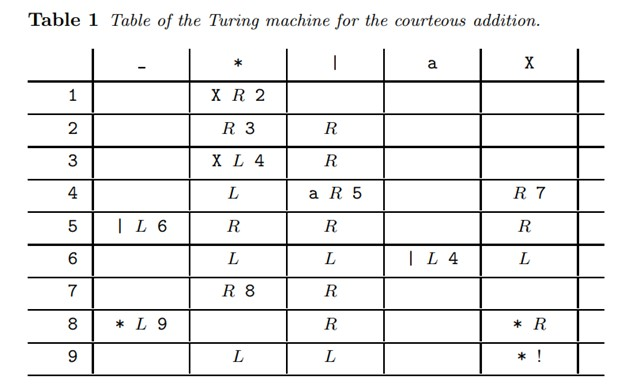
\includegraphics[height = 6cm]{tabla1.jpg}
	\end{figure}
	\section*{Capturas del Funcionamiento}
	En esta sección al igual que en los anteriores programas, se encuentran las capturas de pantalla del funcionamiento del programa.	
	\begin{enumerate}
		\item \textbf{Cadena Manual}
		\begin{itemize}
			\item 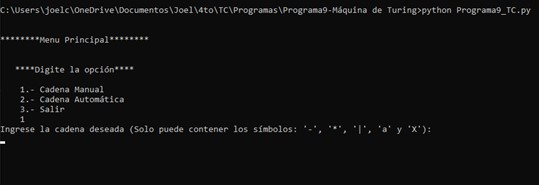
\includegraphics[height = 4cm]{CM1.jpg}
			\item 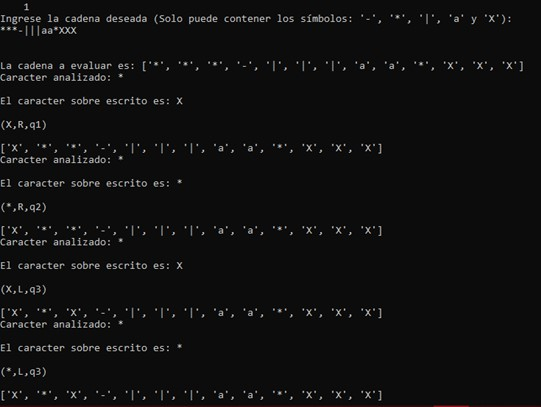
\includegraphics[height = 4cm]{CM2.jpg}
			\item 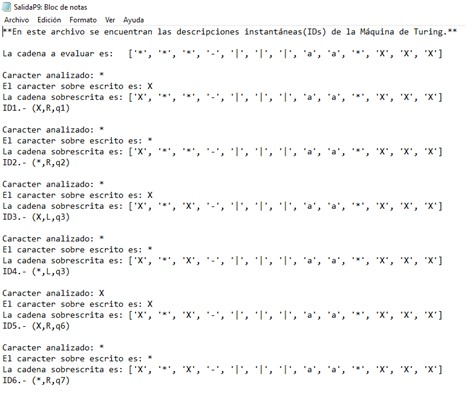
\includegraphics[height = 4cm]{CM3.jpg}
			\item 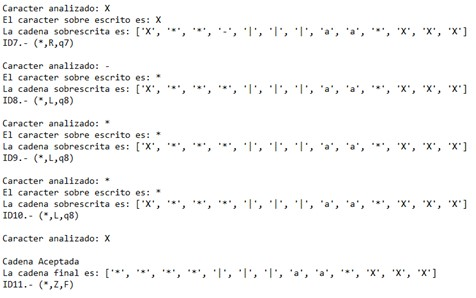
\includegraphics[height = 4cm]{CM4.jpg}
		\end{itemize}				
		\item \textbf{Cadena Automática}
		\begin{itemize}
			\item 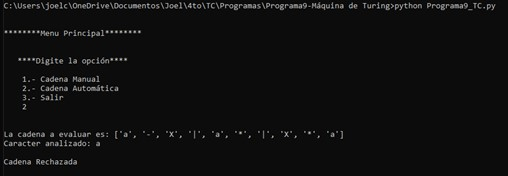
\includegraphics[height = 4cm]{CA1.jpg}
			\item 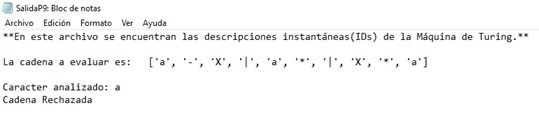
\includegraphics[height = 4cm]{CA2.jpg}
			\item 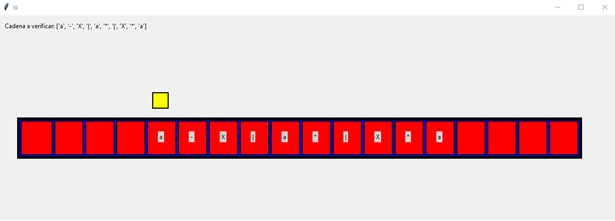
\includegraphics[height = 4cm]{CA3.jpg}
		\end{itemize}	
	\end{enumerate}
	
	\section*{Código}
	\begin{python}
		# Programa 9.Máquina de Turing
		# Nombre: Colín Ramiro Joel
		# Profesor: Juarez Martínez Genaro
		# Grupo: 4CM2
		# Materia: Teoría Computacional
		import sys
		import time
		import random
		from tkinter import*
		from random import randint
		
		def maqTuring(opc):
			archivo = open("SalidaP9.txt","w")
			archivo.write("**En este archivo se encuentran las descripciones instantáneas(IDs) de la Máquina de Turing.**\n\n")
			alfabeto = ["-","*","|","a","X"]
			if(opc == 1):        
				cadena = input("Ingrese la cadena deseada (Solo puede contener los símbolos: '-', '*', '|', 'a' y 'X'): \n")
			elif(opc == 2):
				tamCad = randint(0,100)
				cadena = ""
				for i in range(0, tamCad):
					cadena = cadena + random.choice(alfabeto)            
			cad = []    
			for elem in cadena:
				cad.append(elem)
			print("\n")
			if(len(cad) <= 10):
				ventana = Tk()
				canva = Canvas(ventana , width=1200, height =400)
				ventana.geometry("1200x400")
				canva.pack()
				canva.create_rectangle(39, 200, 1130, 275, width=5, fill='blue')
				xIni = 45
				xFin = 105
				yIni = 205
				yFin = 270
				mens = Label(ventana, text = "Cadena a verificar: " + str(cad)).place(x=10,y=10)
				xCabezaIni = 300
				xCabezaFin = 330
				canva.create_rectangle(xCabezaIni, 150, xCabezaFin, 180, width=2, fill='yellow')  
				caract = ""
				for i in range(0,18):
					canva.create_rectangle(xIni, yIni, xFin, yFin, width=2, fill='red')
					xIni = xFin + 5
					xFin = xFin + 60   
				posxCad = 310
				posyCad = 225  
				for car in cad:
				caract = caract + car 
					caracterAnim = Label(ventana, text=car, bg="light gray").place(x=posxCad,y=posyCad)
					posxCad = posxCad + 60     
			estado = "q0"
			i = 0 
			cont = 1
			print("La cadena a evaluar es: " + str(cad)) 
			archivo.write("La cadena a evaluar es:   " + str(cad) + "\n\n")
			try:        
				while(estado != "q9"):
					pos = 0
					posaux = 0
					for elem in cad:
						if(pos == i):
							pos = pos+1
					if(i == -1):
						cad.insert(0, "")
						i = 0
					if(estado == "q0"): #Estado q0 = 1
						if(cad[i] == "*"):
							print("Caracter analizado: " + cad[i] + "\n")
							archivo.write("Caracter analizado: "+cad[i]+"\n")
							estado = "q1"
							cad[i] = "X"     
							i = i+1                             
							print("El caracter sobre escrito es: X\n")
							archivo.write("El caracter sobre escrito es: X\n")
							print("(X,R,"+estado+")\n")
							print(cad)
							archivo.write("La cadena sobrescrita es: " + str(cad) + "\n")
							archivo.write("ID"+ str(cont) +".- (X,R,"+estado+")\n\n")
							cont = cont+1
						else:
							print("Caracter analizado: " + cad[i] + "\n")
							archivo.write("Caracter analizado: "+cad[i]+"\n")
							estado = "q0"
							cad[i] = i
							print("("+cad[i]+",R,"+estado+")\n")
							print("Cadena Rechazada")                    
							break
				
					if(estado == "q1"): #Estado q1 = 2
						if(cad[i]  == "*"):
							print("Caracter analizado: " + cad[i] + "\n")
							archivo.write("Caracter analizado: "+cad[i]+"\n")
							estado = "q2"
							cad[i] = "*"                    
							i = i+1
							print("El caracter sobre escrito es: *\n")
							archivo.write("El caracter sobre escrito es: *\n")
							print("(*,R,"+estado+")\n")
							print(cad)
							archivo.write("La cadena sobrescrita es: " + str(cad) + "\n")
							archivo.write("ID"+ str(cont) +".- (*,R,"+estado+")\n\n")
							cont = cont+1
						elif(cad[i] == "|"):
							print("Caracter analizado: " + cad[i] + "\n")
							archivo.write("Caracter analizado: "+cad[i]+"\n")
							estado = "q1"
							cad[i] = "|"
							i = i+1
							print("El caracter sobre escrito es: |\n")
							archivo.write("El caracter sobre escrito es: |\n")
							print("(|,R,"+estado+")\n")
							print(cad)
							archivo.write("La cadena sobrescrita es: " + str(cad) + "\n")
							archivo.write("ID"+ str(cont) +".- (|,R,"+estado+")\n\n")
							cont = cont+1
						else:
							print("Caracter analizado: " + cad[i] + "\n")
							archivo.write("Caracter analizado: "+cad[i]+"\n")
							estado = "q1"
							cad[i] = i
							print("("+cad[i]+",Z,"+estado+")\n")
							print("Cadena Rechazada")
							break
					if(estado == "q2"): #Estado q2 = 3
						if(cad[i] == "*"):
							print("Caracter analizado: " + cad[i] + "\n")
							archivo.write("Caracter analizado: "+cad[i]+"\n")
							estado = "q3"
							cad[i] = "X"
							i = i-1
							print("El caracter sobre escrito es: X\n")
							archivo.write("El caracter sobre escrito es: X\n")
							print("(X,L,"+estado+")\n")
							print(cad)
							archivo.write("La cadena sobrescrita es: " + str(cad) + "\n")
							archivo.write("ID"+ str(cont) +".- (X,L,"+estado+")\n\n")
							cont = cont+1
						elif(cad[i] == "|"):
							print("Caracter analizado: " + cad[i] + "\n")
							archivo.write("Caracter analizado: "+cad[i]+"\n")
							estado = "q2"
							cad[i] = "|"
							i = i+1
							print("El caracter sobre escrito es: |\n")
							archivo.write("El caracter sobre escrito es: |\n")
							print("(|,R,"+estado+")\n")
							print(cad)
							archivo.write("La cadena sobrescrita es: " + str(cad) + "\n")
							archivo.write("ID"+ str(cont) +".- (|,R,"+estado+")\n\n")
							cont = cont+1
						else:
							print("Caracter analizado: " + cad[i] + "\n")
							archivo.write("Caracter analizado: "+cad[i]+"\n")
							estado = "q2"
							cad[i] = i
							print("("+cad[i]+",Z,"+estado+")\n")
							print("Cadena Rechazada")
							break     
				
					if(estado == "q3"): #Estado q3 = 4
						if(cad[i] == "*"):
							print("Caracter analizado: " + cad[i] + "\n")
							archivo.write("Caracter analizado: "+cad[i]+"\n")
							estado = "q3"
							cad[i] = "*"
							i = i-1
							print("El caracter sobre escrito es: *\n")
							archivo.write("El caracter sobre escrito es: *\n")
							print("(*,L,"+estado+")\n")
							print(cad)
							archivo.write("La cadena sobrescrita es: " + str(cad) + "\n")
							archivo.write("ID"+ str(cont) +".- (*,L,"+estado+")\n\n")
							cont = cont+1
						elif(cad[i] == "|"):
							print("Caracter analizado: " + cad[i] + "\n")
							archivo.write("Caracter analizado: "+cad[i]+"\n")
							estado = "q4"
							cad[i] = "a"
							i = i+1
							print("El caracter sobre escrito es: a\n")
							archivo.write("El caracter sobre escrito es: a\n")
							print("(a,R,"+estado+")\n")
							print(cad)
							archivo.write("La cadena sobrescrita es: " + str(cad) + "\n")
							archivo.write("ID"+ str(cont) +".- (a,R,"+estado+")\n\n")
							cont = cont+1
						elif(cad[i] == "X"):
							print("Caracter analizado: " + cad[i] + "\n")
							archivo.write("Caracter analizado: "+cad[i]+"\n")
							estado = "q6"
							cad[i] = "X"
							i = i+1
							print("El caracter sobre escrito es: X\n")
							archivo.write("El caracter sobre escrito es: X\n")
							print("(X,R,"+estado+")\n")
							print(cad)
							archivo.write("La cadena sobrescrita es: " + str(cad) + "\n")
							archivo.write("ID"+ str(cont) +".- (X,R,"+estado+")\n\n")
							cont = cont+1
						else:
							print("Caracter analizado: " + cad[i] + "\n")
							archivo.write("Caracter analizado: "+cad[i]+"\n")
							estado = "q3"
							cad[i] = i
							print("("+cad[i]+",Z,"+estado+")\n")
							print("Cadena Rechazada")
							break 
				
					if(estado == "q4"): #Estado q4 = 5
						if(cad[i] == "-"):
							print("Caracter analizado: " + cad[i] + "\n")
							archivo.write("Caracter analizado: "+cad[i]+"\n")
							estado = "q5"
							cad[i] = "|"
							i = i-1
							print("El caracter sobre escrito es: |\n")
							archivo.write("El caracter sobre escrito es: |\n")
							print("(|,L,"+estado+")\n")
							print(cad)
							archivo.write("La cadena sobrescrita es: " + str(cad) + "\n")
							archivo.write("ID"+ str(cont) +".- (|,L,"+estado+")\n\n")
							cont = cont+1
						elif(cad[i] == "*"):
							print("Caracter analizado: " + cad[i] + "\n")
							archivo.write("Caracter analizado: "+cad[i]+"\n")
							estado = "q4"
							cad[i] = "*"
							i = i+1
							print("El caracter sobre escrito es: *\n")
							archivo.write("El caracter sobre escrito es: *\n")
							print("(*,R,"+estado+")\n")
							print(cad)
							archivo.write("La cadena sobrescrita es: " + str(cad) + "\n")
							archivo.write("ID"+ str(cont) +".- (*,R,"+estado+")\n\n")
							cont = cont+1
						elif(cad[i] == "|"):
							print("Caracter analizado: " + cad[i] + "\n")
							archivo.write("Caracter analizado: "+cad[i]+"\n")
							estado = "q4"
							cad[i] = "|"
							i = i+1
							print("El caracter sobre escrito es: |\n")
							archivo.write("El caracter sobre escrito es: |\n")
							print("(|,R,"+estado+")\n")
							print(cad)
							archivo.write("La cadena sobrescrita es: " + str(cad) + "\n")
							archivo.write("ID"+ str(cont) +".- (|,R,"+estado+")\n\n")
							cont = cont+1
						elif(cad[i] == "X"):
							print("Caracter analizado: " + cad[i] + "\n")
							archivo.write("Caracter analizado: "+cad[i]+"\n")
							estado = "q4"
							cad[i] = "X"
							i = i+1
							print("El caracter sobre escrito es: X\n")
							archivo.write("El caracter sobre escrito es: X\n")
							print("(X,R,"+estado+")\n")
							print(cad)
							archivo.write("La cadena sobrescrita es: " + str(cad) + "\n")
							archivo.write("ID"+ str(cont) +".- (X,R,"+estado+")\n\n")
							cont = cont+1
						else:
							print("Caracter analizado: " + cad[i] + "\n")
							archivo.write("Caracter analizado: "+cad[i]+"\n")
							estado = "q4"
							cad[i] = i
							print("("+cad[i]+",Z,"+estado+")\n")
							print("Cadena Rechazada")
							break 
				
					if(estado == "q5"): #Estado q5 = 6
						if(cad[i] == "*"):
							print("Caracter analizado: " + cad[i] + "\n")
							archivo.write("Caracter analizado: "+cad[i]+"\n")
							estado = "q5"
							cad[i] = "*"
							i = i-1
							print("El caracter sobre escrito es: *\n")
							archivo.write("El caracter sobre escrito es: *\n")
							print("(*,L,"+estado+")\n")
							print(cad)
							archivo.write("La cadena sobrescrita es: " + str(cad) + "\n")
							archivo.write("ID"+ str(cont) +".- (*,L,"+estado+")\n\n")
							cont = cont+1
						elif(cad[i] == "|"):
							print("Caracter analizado: " + cad[i] + "\n")
							archivo.write("Caracter analizado: "+cad[i]+"\n")
							estado = "q5"
							cad[i] = "|"
							i = i-1
							print("El caracter sobre escrito es: |\n")
							archivo.write("El caracter sobre escrito es: |\n")
							print("(|,L,"+estado+")\n")
							print(cad)
							archivo.write("La cadena sobrescrita es: " + str(cad) + "\n")
							archivo.write("ID"+ str(cont) +".- (|,L,"+estado+")\n\n")
							cont = cont+1
						elif(cad[i] == "a"):
							print("Caracter analizado: " + cad[i] + "\n")
							archivo.write("Caracter analizado: "+cad[i]+"\n")
							estado = "q3"
							cad[i] = "|"
							i = i-1
							print("El caracter sobre escrito es: |\n")
							archivo.write("El caracter sobre escrito es: |\n")
							print("(|,L,"+estado+")\n")
							print(cad)
							archivo.write("La cadena sobrescrita es: " + str(cad) + "\n")
							archivo.write("ID"+ str(cont) +".- (|,L,"+estado+")\n\n")
							cont = cont+1
						elif(cad[i] == "X"):
							print("Caracter analizado: " + cad[i] + "\n")
							archivo.write("Caracter analizado: "+cad[i]+"\n")
							estado = "q5"
							cad[i] = "X"
							i = i-1
							print("El caracter sobre escrito es: X\n")
							archivo.write("El caracter sobre escrito es: X\n")
							print("(X,L,"+estado+")\n")
							print(cad)
							archivo.write("La cadena sobrescrita es: " + str(cad) + "\n")
							archivo.write("ID"+ str(cont) +".- (X,L,"+estado+")\n\n")
							cont = cont+1
						else:
							print("Caracter analizado: " + cad[i] + "\n")
							archivo.write("Caracter analizado: "+cad[i]+"\n")
							estado = "q5"
							cad[i] = i
							print("("+cad[i]+",Z,"+estado+")\n")
							print("Cadena Rechazada")
							break 
				
					if(estado == "q6"): #Estado q6 = 7
						if(cad[i] == "*"):
							print("Caracter analizado: " + cad[i] + "\n")
							archivo.write("Caracter analizado: "+cad[i]+"\n")
							estado = "q7"
							cad[i] = "*"
							i = i+1
							print("El caracter sobre escrito es: *\n")
							archivo.write("El caracter sobre escrito es: *\n")
							print("(*,R,"+estado+")\n")
							print(cad)
							archivo.write("La cadena sobrescrita es: " + str(cad) + "\n")
							archivo.write("ID"+ str(cont) +".- (*,R,"+estado+")\n\n")
							cont = cont+1
						elif(cad[i] == "|"):
							print("Caracter analizado: " + cad[i] + "\n")
							archivo.write("Caracter analizado: "+cad[i]+"\n")
							estado = "q6"
							cad[i] = "|"
							i = i+1
							print("El caracter sobre escrito es: |\n")
							archivo.write("El caracter sobre escrito es: |\n")
							print("(|,R,"+estado+")\n")
							print(cad)
							archivo.write("La cadena sobrescrita es: " + str(cad) + "\n")
							archivo.write("ID"+ str(cont) +".- (|,R,"+estado+")\n\n")
							cont = cont+1
						else:
							print("Caracter analizado: " + cad[i] + "\n")
							archivo.write("Caracter analizado: "+cad[i]+"\n")
							estado = "q6"
							cad[i] = i
							print("("+cad[i]+",Z,"+estado+")\n")
							print("Cadena Rechazada")
							break    
				
					if(estado == "q7"): #Estado q7 = 8
						if(cad[i] == "-"):
							print("Caracter analizado: " + cad[i] + "\n")
							archivo.write("Caracter analizado: "+cad[i]+"\n")
							estado = "q8"
							cad[i] = "*"
							i = i-1
							print("El caracter sobre escrito es: *\n")
							archivo.write("El caracter sobre escrito es: *\n")
							print("(*,L,"+estado+")\n")
							print(cad)
							archivo.write("La cadena sobrescrita es: " + str(cad) + "\n")
							archivo.write("ID"+ str(cont) +".- (*,L,"+estado+")\n\n")
							cont = cont+1
						elif(cad[i] == "|"):
							print("Caracter analizado: " + cad[i] + "\n")
							archivo.write("Caracter analizado: "+cad[i]+"\n")
							estado = "q7"
							cad[i] = "|"
							i = i+1
							print("El caracter sobre escrito es: |\n")
							archivo.write("El caracter sobre escrito es: |\n")
							print("(|,R,"+estado+")\n")
							print(cad)
							archivo.write("La cadena sobrescrita es: " + str(cad) + "\n")
							archivo.write("ID"+ str(cont) +".- (|,R,"+estado+")\n\n")
							cont = cont+1
						elif(cad[i] == "X"):
							print("Caracter analizado: " + cad[i] + "\n")
							archivo.write("Caracter analizado: "+cad[i]+"\n")
							estado = "q7"
							cad[i] = "*"
							i = i+1
							print("El caracter sobre escrito es: X\n")
							archivo.write("El caracter sobre escrito es: X\n")
							print("(*,R,"+estado+")\n")
							print(cad)
							archivo.write("La cadena sobrescrita es: " + str(cad) + "\n")
							archivo.write("ID"+ str(cont) +".- (*,R,"+estado+")\n\n")
							cont = cont+1
						else:
							print("Caracter analizado: " + cad[i] + "\n")
							archivo.write("Caracter analizado: "+cad[i]+"\n")
							estado = "q7"
							cad[i] = i
							print("("+cad[i]+",Z,"+estado+")\n")
							print("Cadena Rechazada")
							break 
				
					if(estado == "q8"): #Estado q8 = 9
						if(cad[i] == "*"):
							print("Caracter analizado: " + cad[i] + "\n")
							archivo.write("Caracter analizado: "+cad[i]+"\n")
							estado = "q8"
							cad[i] = "*"
							i = i-1
							print("El caracter sobre escrito es: *\n")
							archivo.write("El caracter sobre escrito es: *\n")
							print("(*,L,"+estado+")\n")
							print(cad)
							archivo.write("La cadena sobrescrita es: " + str(cad) + "\n")
							archivo.write("ID"+ str(cont) +".- (*,L,"+estado+")\n\n")
							cont = cont+1
						elif(cad[i] == "|"):
							print("Caracter analizado: " + cad[i] + "\n")
							archivo.write("Caracter analizado: "+cad[i]+"\n")
							estado = "q8"
							cad[i] = "*"
							i = i-1
							print("El caracter sobre escrito es: *\n")
							archivo.write("El caracter sobre escrito es: *\n")
							print("(*,L,"+estado+")\n")
							print(cad)
							archivo.write("La cadena sobrescrita es: " + str(cad) + "\n")
							archivo.write("ID"+ str(cont) +".- (*,L,"+estado+")\n\n")
							cont = cont+1
						elif(cad[i] == "X"):
							print("Caracter analizado: " + cad[i] + "\n")
							archivo.write("Caracter analizado: "+cad[i]+"\n")
							cad[i] = "*"
							print("\nCadena Aceptada\n")
							archivo.write("\nCadena Aceptada\n")
							print("(*,Z,F)"+"\n")
							print(cad)
							archivo.write("La cadena final es: " + str(cad) + "\n")
							archivo.write("ID"+ str(cont) +".- (*,Z,F)"+"\n\n")
							cont = cont+1
							break
						else:
							estado = "q8"
							cad[i] = i
							print("("+cad[i]+",Z,"+estado+")\n")
							print("Cadena Rechazada")
							break 
			except:
				print("Cadena Rechazada")
		
		opc = 0
		salir = 3
		while opc != salir:
			print("\n\n********Menu Principal********\n\n")
			print("   ****Digite la opción****")
			opc = int(input('''
			1.- Cadena Manual
			2.- Cadena Automática
			3.- Salir
			'''))    
			if(opc == 1) or (opc == 2):
				maqTuring(opc)
			elif opc == 3:
				print("Saliendo del Programa. Hasta Luego!!!!")
			else:
				print("Opcion inválida, Vuelva a intentar")
	\end{python}
	
	\section*{Conclusiones}
	Para concluir con este noveno y último programa quiero destacar que intenté aplicar todos los conocimientos adquiridos a lo largo del curso, más que nada lo de los AFD.
	
	Este programa en particular me resultó algo complicado de entender, ya que no lograba comprender al 100 por ciento el funcionamiento de una Máquina de Turing, sin embargo, despues de revisar algunos tutoriales y repasar el PDF proporcionado por el profesor asi como que de otros docuemntos en la red,  logré comprender y realizar el análisis del programa. 
	
	En cuanto al programa en si puedo concluir que este tema de la Máquina de Turing es de los más sino es que el más importante en la computación. Es fundamental la comprensión de este tema ya que a un nivel de extracción, llega a ser las bases de practicamente todo.
	
	Concluyo que ha sido un buen curso, a mi parecer al que más le he sacado provecho en cuanto a aprendizaje y en cuanto a práctica. No cabe duda que aun faltan muchas cosas por mejorar aprender y sobre todo de realizar un análisis previo para entender de lo que se está hablando.
	
	
	\section*{Referencias}
	\begin{enumerate}
		\item INAOE. (2017). Máquinas de Turing. Diciembre 21,2021, de INAOE Sitio web: https://ccc.inaoep.mx/~emorales/Cursos/Automatas/IntroMaquinasTuring.pdf
		\item Bootcamp AI. (2021). Máquinas de Turing. Diciembre 21,2021, de Bootcamp AI Sitio web: https://bootcampai.medium.com/
		\item UANL. (1996). MÁQUINAS DE TURING. Diciembre 21,2021, de UANL Sitio web: http://www.itnuevolaredo.edu.mx/takeyas/apuntes/Automatas/Apuntes/turing.pdf
	\end{enumerate}
\end{document}